\documentclass[aspectratio=169,11pt]{beamer}
% =====================================================================
%  pds-beamer.tex — Estilo común de las transparencias.
%
%  Uso (desde teoría/Tx/transparencias/):
%     \documentclass[aspectratio=169,11pt]{beamer}
%     % =====================================================================
%  pds-beamer.tex — Estilo común de las transparencias.
%
%  Uso (desde teoría/Tx/transparencias/):
%     \documentclass[aspectratio=169,11pt]{beamer}
%     % =====================================================================
%  pds-beamer.tex — Estilo común de las transparencias.
%
%  Uso (desde teoría/Tx/transparencias/):
%     \documentclass[aspectratio=169,11pt]{beamer}
%     \input{../../comun/pds-beamer}
%     \title{...}  \subtitle{Tema x · ...}
%     \begin{document}
%       \portada
%       ...
%     \end{document}
%  Compilar con:  latexmk -xelatex  (o «make» desde teoría/)
% =====================================================================

\usetheme{Boadilla}
\usecolortheme{orchid}
\usefonttheme{professionalfonts}
\setbeamercovered{transparent}
\setbeamersize{text margin left=0.8cm, text margin right=0.8cm}
\setbeamertemplate{navigation symbols}{}
\setbeamertemplate{itemize item}[square]
\setbeamertemplate{itemize subitem}[circle]
\setbeamertemplate{itemize subsubitem}[triangle]
\setbeamertemplate{enumerate item}[square]
\setbeamertemplate{enumerate subitem}[circle]
\setbeamertemplate{caption}{\raggedright\insertcaption\par}

\input{../../comun/pds-comun.tex}

% Tipografía: Fira Sans + Fira Math (legibles en proyector)
\usepackage{fontspec}
\usepackage{unicode-math}
% Se cargan por nombre de fichero para que funcionen con cualquier
% instalación de TeX Live (o MiKTeX) sin instalar fuentes en el sistema.
\setmainfont{FiraSans}[Extension=.otf, UprightFont=*-Regular, BoldFont=*-SemiBold,
  ItalicFont=*-Italic, BoldItalicFont=*-SemiBoldItalic]
\setsansfont{FiraSans}[Extension=.otf, UprightFont=*-Regular, BoldFont=*-SemiBold,
  ItalicFont=*-Italic, BoldItalicFont=*-SemiBoldItalic]
\setmonofont{FiraMono}[Extension=.otf, UprightFont=*-Regular, BoldFont=*-Medium, AutoFakeSlant=0.15, Scale=0.92]
\setmathfont{FiraMath-Regular.otf}
\setmathfont{latinmodern-math.otf}[range={"229B,"22EE,"22F1}]

% Colores del tema ajustados a la paleta común (más contraste)
\setbeamercolor{structure}{fg=pdsazul}
\setbeamercolor{alerted text}{fg=pdsrojo}
\setbeamercolor{example text}{fg=pdsverde}
\setbeamercolor{block title}{bg=pdsazul, fg=white}
\setbeamercolor{block body}{bg=pdsfondo}
\setbeamercolor{block title alerted}{bg=pdsrojo, fg=white}
\setbeamercolor{block body alerted}{bg=pdsrojo!6}
\setbeamercolor{block title example}{bg=pdsverde, fg=white}
\setbeamercolor{block body example}{bg=pdsverde!6}
\setbeamercolor{frametitle}{fg=pdsazul, bg=white}
\setbeamerfont{frametitle}{size=\large, series=\bfseries}
\setbeamerfont{block title}{size=\normalsize, series=\bfseries}
\setbeamertemplate{blocks}[rounded][shadow=false]

% Logo en la esquina superior derecha de cada transparencia
\pgfdeclareimage[height=0.8cm]{logo}{../../comun/ucm.png}
\addtobeamertemplate{frametitle}{}{%
  \begin{tikzpicture}[remember picture, overlay]
    \node[anchor=north east, inner sep=0pt] at ([xshift=-0.25cm, yshift=-0.2cm]current page.north east) {\pgfuseimage{logo}};
  \end{tikzpicture}}

% Datos de portada
\author[\autorescorto]{\autores}
\institute[UCM]{\footnotesize\departamento\\\universidad}
\date[\curso]{\footnotesize\grado\\\curso}

\newcommand{\portada}{%
  \begin{frame}[plain]
    \begin{center}
      
\includegraphics[height=1.9cm]{../../comun/ucm.png}
    \end{center}
    \vspace{-0.4cm}
    \titlepage
  \end{frame}}

% Índice al empezar cada sección
\AtBeginSection[]{%
  \begin{frame}{Contenido}
    \tableofcontents[currentsection, hideothersubsections]
  \end{frame}}

\renewcommand{\pdscodesize}{\scriptsize}

% Utilidades
% \herramienta{T1-convolucion-continua}: enlace a la página publicada de
% herramientas/html (se abre en el navegador, sin instalar nada).
% \herramientaservidor{server/....py}: app que necesita Python (bokeh serve).
\newcommand{\urlherramientas}{https://ucm-237.github.io/PdS/}
\newcommand{\herramienta}[1]{%
  \par\vfill\hfill{\scriptsize\color{pdsgris}\faIcon\ \href{\urlherramientas#1.html}{Herramienta interactiva: \texttt{#1}}}}
\newcommand{\herramientaservidor}[1]{%
  \par\vfill\hfill{\scriptsize\color{pdsgris}\faIcon\ Herramienta interactiva (con Python): \texttt{herramientas/#1}}}
\newcommand{\faIcon}{\textbf{▶}}
\newcommand{\gris}[1]{{\color{pdsgris}#1}}
\newcommand{\nota}[1]{\par\vspace{2pt}{\footnotesize\color{pdsgris}\textit{#1}}\par}
% Nota sobre una errata de versiones anteriores (solo con \ERRATAS)
\newcommand{\errata}[1]{\iferratas\nota{Errata de versiones anteriores: #1}\fi}
\newcommand{\apuntes}[1]{\nota{Más detalle en los apuntes, #1.}}

% Bloques con nombre en castellano
\newenvironment{definicion}[1][Definición]{\begin{block}{#1}}{\end{block}}
\newenvironment{importante}[1][Importante]{\begin{alertblock}{#1}}{\end{alertblock}}
\newenvironment{ejemplo}[1][Ejemplo]{\begin{exampleblock}{#1}}{\end{exampleblock}}

%     \title{...}  \subtitle{Tema x · ...}
%     \begin{document}
%       \portada
%       ...
%     \end{document}
%  Compilar con:  latexmk -xelatex  (o «make» desde teoría/)
% =====================================================================

\usetheme{Boadilla}
\usecolortheme{orchid}
\usefonttheme{professionalfonts}
\setbeamercovered{transparent}
\setbeamersize{text margin left=0.8cm, text margin right=0.8cm}
\setbeamertemplate{navigation symbols}{}
\setbeamertemplate{itemize item}[square]
\setbeamertemplate{itemize subitem}[circle]
\setbeamertemplate{itemize subsubitem}[triangle]
\setbeamertemplate{enumerate item}[square]
\setbeamertemplate{enumerate subitem}[circle]
\setbeamertemplate{caption}{\raggedright\insertcaption\par}

% =====================================================================
%  pds-comun.tex — Paquetes, colores y estilos de código comunes a
%  transparencias, apuntes y hojas de ejercicios. Compilar con XeLaTeX.
%  No cargar directamente: lo cargan pds-beamer.tex y pds-apuntes.tex.
% =====================================================================

\usepackage{polyglossia}
\setmainlanguage{spanish}
\usepackage{mathtools}
\usepackage{graphicx}
\usepackage{booktabs}
\usepackage{multirow}
\usepackage{array}
\usepackage{xcolor}
\usepackage{tikz}
\usetikzlibrary{positioning,arrows.meta,calc,shapes.geometric,decorations.pathreplacing}
\usepackage{listings}
\usepackage{siunitx}
\sisetup{output-decimal-marker={,}, group-separator={\,}, per-mode=symbol}

% Notas de erratas de versiones anteriores: no se imprimen salvo que se
% defina \ERRATAS antes de cargar el estilo (make ERRATAS=1)
\newif\iferratas
\ifdefined\ERRATAS \erratastrue \fi

% Ruta común (logo y figuras compartidas)
\providecommand{\rutacomun}{../../comun/}
\input{\rutacomun datos.tex}

% ---------------------------------------------------------------------
%  Paleta (la misma que usan las figuras generadas con Python,
%  ver comun/pds_estilo.py)
% ---------------------------------------------------------------------
\definecolor{pdsazul}{HTML}{2B3A8C}
\definecolor{pdsrojo}{HTML}{C0392B}
\definecolor{pdsverde}{HTML}{1E7B4F}
\definecolor{pdsnaranja}{HTML}{D9822B}
\definecolor{pdsgris}{HTML}{5A5A66}
\definecolor{pdsfondo}{HTML}{F3F4FA}
\definecolor{pdscodigo}{HTML}{F7F7F2}

% ---------------------------------------------------------------------
%  Diagramas de bloques (TikZ)
% ---------------------------------------------------------------------
\tikzset{
  bloque/.style={rectangle, rounded corners=2pt, draw=pdsazul!80, fill=pdsfondo,
                 very thick, minimum height=8mm, minimum width=14mm, align=center},
  sumador/.style={circle, draw=pdsazul!80, fill=pdsfondo, thick, inner sep=1.5pt},
  flecha/.style={-{Stealth[length=2.2mm]}, thick, pdsgris},
}

% ---------------------------------------------------------------------
%  Código: Python y Matlab en paralelo
% ---------------------------------------------------------------------
\newcommand{\pdscodesize}{\footnotesize}
\lstdefinestyle{pds}{
  basicstyle=\ttfamily\pdscodesize,
  keywordstyle=\color{pdsazul}\bfseries,
  commentstyle=\color{pdsverde}\itshape,
  stringstyle=\color{pdsrojo},
  numbers=none,
  backgroundcolor=\color{pdscodigo},
  frame=single, rulecolor=\color{pdsgris!40}, framerule=0.4pt,
  xleftmargin=2pt, xrightmargin=2pt, aboveskip=2pt, belowskip=2pt,
  columns=fullflexible, keepspaces=true,
  showstringspaces=false, breaklines=true, tabsize=4,
  upquote=true,
  % Con XeLaTeX, listings desordena los caracteres no ASCII junto a
  % dígitos («2π» sale «π2»): se sustituyen por su versión matemática.
  literate={π}{{$\pi$}}1 {δ}{{$\delta$}}1 {ω}{{$\omega$}}1 {Ω}{{$\Omega$}}1
           {≈}{{$\approx$}}1 {µ}{{$\mu$}}1 {·}{{$\cdot$}}1 {α}{{$\alpha$}}1
           {á}{{á}}1 {é}{{é}}1 {í}{{í}}1 {ó}{{ó}}1 {ú}{{ú}}1 {ñ}{{ñ}}1 {¿}{{¿}}1,
}
\lstdefinestyle{python}{style=pds, language=Python,
  morekeywords={as,True,False,None}}
\lstdefinestyle{matlab}{style=pds, language=Matlab,
  morekeywords={function,end,true,false}}

% \codigo{<ruta sin extensión>} muestra el mismo ejemplo en Python
% y en Matlab, uno al lado del otro. Los ficheros viven en
% ../codigo/python/<nombre>.py y ../codigo/matlab/<nombre>.m y se
% ejecutan en las pruebas (make prueba-codigo).
\newcommand{\rutacodigo}{../codigo/}
\newcommand{\codigoetiqueta}[1]{{\sffamily\scriptsize\bfseries\color{pdsgris}#1}}
\newcommand{\codigo}[2][]{%
  \par\noindent
  \begin{minipage}[t]{0.495\linewidth}
    \codigoetiqueta{Python}\par\vspace{1pt}
    \lstinputlisting[style=python,#1]{\rutacodigo python/#2.py}
  \end{minipage}\hfill
  \begin{minipage}[t]{0.495\linewidth}
    \codigoetiqueta{Matlab}\par\vspace{1pt}
    \lstinputlisting[style=matlab,#1]{\rutacodigo matlab/#2.m}
  \end{minipage}\par}

\input{\rutacomun notacion.tex}


% Tipografía: Fira Sans + Fira Math (legibles en proyector)
\usepackage{fontspec}
\usepackage{unicode-math}
% Se cargan por nombre de fichero para que funcionen con cualquier
% instalación de TeX Live (o MiKTeX) sin instalar fuentes en el sistema.
\setmainfont{FiraSans}[Extension=.otf, UprightFont=*-Regular, BoldFont=*-SemiBold,
  ItalicFont=*-Italic, BoldItalicFont=*-SemiBoldItalic]
\setsansfont{FiraSans}[Extension=.otf, UprightFont=*-Regular, BoldFont=*-SemiBold,
  ItalicFont=*-Italic, BoldItalicFont=*-SemiBoldItalic]
\setmonofont{FiraMono}[Extension=.otf, UprightFont=*-Regular, BoldFont=*-Medium, AutoFakeSlant=0.15, Scale=0.92]
\setmathfont{FiraMath-Regular.otf}
\setmathfont{latinmodern-math.otf}[range={"229B,"22EE,"22F1}]

% Colores del tema ajustados a la paleta común (más contraste)
\setbeamercolor{structure}{fg=pdsazul}
\setbeamercolor{alerted text}{fg=pdsrojo}
\setbeamercolor{example text}{fg=pdsverde}
\setbeamercolor{block title}{bg=pdsazul, fg=white}
\setbeamercolor{block body}{bg=pdsfondo}
\setbeamercolor{block title alerted}{bg=pdsrojo, fg=white}
\setbeamercolor{block body alerted}{bg=pdsrojo!6}
\setbeamercolor{block title example}{bg=pdsverde, fg=white}
\setbeamercolor{block body example}{bg=pdsverde!6}
\setbeamercolor{frametitle}{fg=pdsazul, bg=white}
\setbeamerfont{frametitle}{size=\large, series=\bfseries}
\setbeamerfont{block title}{size=\normalsize, series=\bfseries}
\setbeamertemplate{blocks}[rounded][shadow=false]

% Logo en la esquina superior derecha de cada transparencia
\pgfdeclareimage[height=0.8cm]{logo}{../../comun/ucm.png}
\addtobeamertemplate{frametitle}{}{%
  \begin{tikzpicture}[remember picture, overlay]
    \node[anchor=north east, inner sep=0pt] at ([xshift=-0.25cm, yshift=-0.2cm]current page.north east) {\pgfuseimage{logo}};
  \end{tikzpicture}}

% Datos de portada
\author[\autorescorto]{\autores}
\institute[UCM]{\footnotesize\departamento\\\universidad}
\date[\curso]{\footnotesize\grado\\\curso}

\newcommand{\portada}{%
  \begin{frame}[plain]
    \begin{center}
      
\includegraphics[height=1.9cm]{../../comun/ucm.png}
    \end{center}
    \vspace{-0.4cm}
    \titlepage
  \end{frame}}

% Índice al empezar cada sección
\AtBeginSection[]{%
  \begin{frame}{Contenido}
    \tableofcontents[currentsection, hideothersubsections]
  \end{frame}}

\renewcommand{\pdscodesize}{\scriptsize}

% Utilidades
% \herramienta{T1-convolucion-continua}: enlace a la página publicada de
% herramientas/html (se abre en el navegador, sin instalar nada).
% \herramientaservidor{server/....py}: app que necesita Python (bokeh serve).
\newcommand{\urlherramientas}{https://ucm-237.github.io/PdS/}
\newcommand{\herramienta}[1]{%
  \par\vfill\hfill{\scriptsize\color{pdsgris}\faIcon\ \href{\urlherramientas#1.html}{Herramienta interactiva: \texttt{#1}}}}
\newcommand{\herramientaservidor}[1]{%
  \par\vfill\hfill{\scriptsize\color{pdsgris}\faIcon\ Herramienta interactiva (con Python): \texttt{herramientas/#1}}}
\newcommand{\faIcon}{\textbf{▶}}
\newcommand{\gris}[1]{{\color{pdsgris}#1}}
\newcommand{\nota}[1]{\par\vspace{2pt}{\footnotesize\color{pdsgris}\textit{#1}}\par}
% Nota sobre una errata de versiones anteriores (solo con \ERRATAS)
\newcommand{\errata}[1]{\iferratas\nota{Errata de versiones anteriores: #1}\fi}
\newcommand{\apuntes}[1]{\nota{Más detalle en los apuntes, #1.}}

% Bloques con nombre en castellano
\newenvironment{definicion}[1][Definición]{\begin{block}{#1}}{\end{block}}
\newenvironment{importante}[1][Importante]{\begin{alertblock}{#1}}{\end{alertblock}}
\newenvironment{ejemplo}[1][Ejemplo]{\begin{exampleblock}{#1}}{\end{exampleblock}}

%     \title{...}  \subtitle{Tema x · ...}
%     \begin{document}
%       \portada
%       ...
%     \end{document}
%  Compilar con:  latexmk -xelatex  (o «make» desde teoría/)
% =====================================================================

\usetheme{Boadilla}
\usecolortheme{orchid}
\usefonttheme{professionalfonts}
\setbeamercovered{transparent}
\setbeamersize{text margin left=0.8cm, text margin right=0.8cm}
\setbeamertemplate{navigation symbols}{}
\setbeamertemplate{itemize item}[square]
\setbeamertemplate{itemize subitem}[circle]
\setbeamertemplate{itemize subsubitem}[triangle]
\setbeamertemplate{enumerate item}[square]
\setbeamertemplate{enumerate subitem}[circle]
\setbeamertemplate{caption}{\raggedright\insertcaption\par}

% =====================================================================
%  pds-comun.tex — Paquetes, colores y estilos de código comunes a
%  transparencias, apuntes y hojas de ejercicios. Compilar con XeLaTeX.
%  No cargar directamente: lo cargan pds-beamer.tex y pds-apuntes.tex.
% =====================================================================

\usepackage{polyglossia}
\setmainlanguage{spanish}
\usepackage{mathtools}
\usepackage{graphicx}
\usepackage{booktabs}
\usepackage{multirow}
\usepackage{array}
\usepackage{xcolor}
\usepackage{tikz}
\usetikzlibrary{positioning,arrows.meta,calc,shapes.geometric,decorations.pathreplacing}
\usepackage{listings}
\usepackage{siunitx}
\sisetup{output-decimal-marker={,}, group-separator={\,}, per-mode=symbol}

% Notas de erratas de versiones anteriores: no se imprimen salvo que se
% defina \ERRATAS antes de cargar el estilo (make ERRATAS=1)
\newif\iferratas
\ifdefined\ERRATAS \erratastrue \fi

% Ruta común (logo y figuras compartidas)
\providecommand{\rutacomun}{../../comun/}
\input{\rutacomun datos.tex}

% ---------------------------------------------------------------------
%  Paleta (la misma que usan las figuras generadas con Python,
%  ver comun/pds_estilo.py)
% ---------------------------------------------------------------------
\definecolor{pdsazul}{HTML}{2B3A8C}
\definecolor{pdsrojo}{HTML}{C0392B}
\definecolor{pdsverde}{HTML}{1E7B4F}
\definecolor{pdsnaranja}{HTML}{D9822B}
\definecolor{pdsgris}{HTML}{5A5A66}
\definecolor{pdsfondo}{HTML}{F3F4FA}
\definecolor{pdscodigo}{HTML}{F7F7F2}

% ---------------------------------------------------------------------
%  Diagramas de bloques (TikZ)
% ---------------------------------------------------------------------
\tikzset{
  bloque/.style={rectangle, rounded corners=2pt, draw=pdsazul!80, fill=pdsfondo,
                 very thick, minimum height=8mm, minimum width=14mm, align=center},
  sumador/.style={circle, draw=pdsazul!80, fill=pdsfondo, thick, inner sep=1.5pt},
  flecha/.style={-{Stealth[length=2.2mm]}, thick, pdsgris},
}

% ---------------------------------------------------------------------
%  Código: Python y Matlab en paralelo
% ---------------------------------------------------------------------
\newcommand{\pdscodesize}{\footnotesize}
\lstdefinestyle{pds}{
  basicstyle=\ttfamily\pdscodesize,
  keywordstyle=\color{pdsazul}\bfseries,
  commentstyle=\color{pdsverde}\itshape,
  stringstyle=\color{pdsrojo},
  numbers=none,
  backgroundcolor=\color{pdscodigo},
  frame=single, rulecolor=\color{pdsgris!40}, framerule=0.4pt,
  xleftmargin=2pt, xrightmargin=2pt, aboveskip=2pt, belowskip=2pt,
  columns=fullflexible, keepspaces=true,
  showstringspaces=false, breaklines=true, tabsize=4,
  upquote=true,
  % Con XeLaTeX, listings desordena los caracteres no ASCII junto a
  % dígitos («2π» sale «π2»): se sustituyen por su versión matemática.
  literate={π}{{$\pi$}}1 {δ}{{$\delta$}}1 {ω}{{$\omega$}}1 {Ω}{{$\Omega$}}1
           {≈}{{$\approx$}}1 {µ}{{$\mu$}}1 {·}{{$\cdot$}}1 {α}{{$\alpha$}}1
           {á}{{á}}1 {é}{{é}}1 {í}{{í}}1 {ó}{{ó}}1 {ú}{{ú}}1 {ñ}{{ñ}}1 {¿}{{¿}}1,
}
\lstdefinestyle{python}{style=pds, language=Python,
  morekeywords={as,True,False,None}}
\lstdefinestyle{matlab}{style=pds, language=Matlab,
  morekeywords={function,end,true,false}}

% \codigo{<ruta sin extensión>} muestra el mismo ejemplo en Python
% y en Matlab, uno al lado del otro. Los ficheros viven en
% ../codigo/python/<nombre>.py y ../codigo/matlab/<nombre>.m y se
% ejecutan en las pruebas (make prueba-codigo).
\newcommand{\rutacodigo}{../codigo/}
\newcommand{\codigoetiqueta}[1]{{\sffamily\scriptsize\bfseries\color{pdsgris}#1}}
\newcommand{\codigo}[2][]{%
  \par\noindent
  \begin{minipage}[t]{0.495\linewidth}
    \codigoetiqueta{Python}\par\vspace{1pt}
    \lstinputlisting[style=python,#1]{\rutacodigo python/#2.py}
  \end{minipage}\hfill
  \begin{minipage}[t]{0.495\linewidth}
    \codigoetiqueta{Matlab}\par\vspace{1pt}
    \lstinputlisting[style=matlab,#1]{\rutacodigo matlab/#2.m}
  \end{minipage}\par}

\input{\rutacomun notacion.tex}


% Tipografía: Fira Sans + Fira Math (legibles en proyector)
\usepackage{fontspec}
\usepackage{unicode-math}
% Se cargan por nombre de fichero para que funcionen con cualquier
% instalación de TeX Live (o MiKTeX) sin instalar fuentes en el sistema.
\setmainfont{FiraSans}[Extension=.otf, UprightFont=*-Regular, BoldFont=*-SemiBold,
  ItalicFont=*-Italic, BoldItalicFont=*-SemiBoldItalic]
\setsansfont{FiraSans}[Extension=.otf, UprightFont=*-Regular, BoldFont=*-SemiBold,
  ItalicFont=*-Italic, BoldItalicFont=*-SemiBoldItalic]
\setmonofont{FiraMono}[Extension=.otf, UprightFont=*-Regular, BoldFont=*-Medium, AutoFakeSlant=0.15, Scale=0.92]
\setmathfont{FiraMath-Regular.otf}
\setmathfont{latinmodern-math.otf}[range={"229B,"22EE,"22F1}]

% Colores del tema ajustados a la paleta común (más contraste)
\setbeamercolor{structure}{fg=pdsazul}
\setbeamercolor{alerted text}{fg=pdsrojo}
\setbeamercolor{example text}{fg=pdsverde}
\setbeamercolor{block title}{bg=pdsazul, fg=white}
\setbeamercolor{block body}{bg=pdsfondo}
\setbeamercolor{block title alerted}{bg=pdsrojo, fg=white}
\setbeamercolor{block body alerted}{bg=pdsrojo!6}
\setbeamercolor{block title example}{bg=pdsverde, fg=white}
\setbeamercolor{block body example}{bg=pdsverde!6}
\setbeamercolor{frametitle}{fg=pdsazul, bg=white}
\setbeamerfont{frametitle}{size=\large, series=\bfseries}
\setbeamerfont{block title}{size=\normalsize, series=\bfseries}
\setbeamertemplate{blocks}[rounded][shadow=false]

% Logo en la esquina superior derecha de cada transparencia
\pgfdeclareimage[height=0.8cm]{logo}{../../comun/ucm.png}
\addtobeamertemplate{frametitle}{}{%
  \begin{tikzpicture}[remember picture, overlay]
    \node[anchor=north east, inner sep=0pt] at ([xshift=-0.25cm, yshift=-0.2cm]current page.north east) {\pgfuseimage{logo}};
  \end{tikzpicture}}

% Datos de portada
\author[\autorescorto]{\autores}
\institute[UCM]{\footnotesize\departamento\\\universidad}
\date[\curso]{\footnotesize\grado\\\curso}

\newcommand{\portada}{%
  \begin{frame}[plain]
    \begin{center}
      
\includegraphics[height=1.9cm]{../../comun/ucm.png}
    \end{center}
    \vspace{-0.4cm}
    \titlepage
  \end{frame}}

% Índice al empezar cada sección
\AtBeginSection[]{%
  \begin{frame}{Contenido}
    \tableofcontents[currentsection, hideothersubsections]
  \end{frame}}

\renewcommand{\pdscodesize}{\scriptsize}

% Utilidades
% \herramienta{T1-convolucion-continua}: enlace a la página publicada de
% herramientas/html (se abre en el navegador, sin instalar nada).
% \herramientaservidor{server/....py}: app que necesita Python (bokeh serve).
\newcommand{\urlherramientas}{https://ucm-237.github.io/PdS/}
\newcommand{\herramienta}[1]{%
  \par\vfill\hfill{\scriptsize\color{pdsgris}\faIcon\ \href{\urlherramientas#1.html}{Herramienta interactiva: \texttt{#1}}}}
\newcommand{\herramientaservidor}[1]{%
  \par\vfill\hfill{\scriptsize\color{pdsgris}\faIcon\ Herramienta interactiva (con Python): \texttt{herramientas/#1}}}
\newcommand{\faIcon}{\textbf{▶}}
\newcommand{\gris}[1]{{\color{pdsgris}#1}}
\newcommand{\nota}[1]{\par\vspace{2pt}{\footnotesize\color{pdsgris}\textit{#1}}\par}
% Nota sobre una errata de versiones anteriores (solo con \ERRATAS)
\newcommand{\errata}[1]{\iferratas\nota{Errata de versiones anteriores: #1}\fi}
\newcommand{\apuntes}[1]{\nota{Más detalle en los apuntes, #1.}}

% Bloques con nombre en castellano
\newenvironment{definicion}[1][Definición]{\begin{block}{#1}}{\end{block}}
\newenvironment{importante}[1][Importante]{\begin{alertblock}{#1}}{\end{alertblock}}
\newenvironment{ejemplo}[1][Ejemplo]{\begin{exampleblock}{#1}}{\end{exampleblock}}

\graphicspath{{../figuras/}}

\title[T5 · Wavelets]{Aplicaciones}
\subtitle{Tema 5 · Parte 2: análisis con wavelets}

\begin{document}
\portada

% =====================================================================
\section{De la STFT a las wavelets}

\begin{frame}{Limitaciones de la STFT}
  \begin{columns}[c]
    \begin{column}{0.46\textwidth}
      \small
      \begin{itemize}
        \item La ventana se elige antes de analizar y es la misma en todas las frecuencias.
        \item Muchas señales tienen \alert{componentes lentas y largas} (tendencias, tonos graves) y \alert{detalles rápidos y breves} (clics, bordes, saltos).
        \item Lo natural es una ventana larga para las bajas frecuencias y corta para las altas: misma cantidad de \emph{periodos} en cada análisis.
        \item Y no siempre una sinusoide es la mejor forma con la que comparar: un latido o un escalón se parecen más a otras ondas.
      \end{itemize}
    \end{column}
    \begin{column}{0.52\textwidth}
      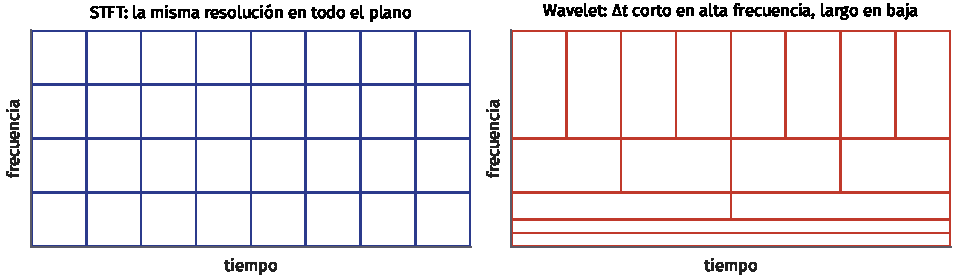
\includegraphics[width=\linewidth]{teselas}
      \nota{Cada rectángulo tiene la misma área $\Delta t\,\Delta f$: el principio de incertidumbre se sigue cumpliendo.}
    \end{column}
  \end{columns}
\end{frame}

\begin{frame}{Wavelets: pequeñas ondas}
  \begin{center}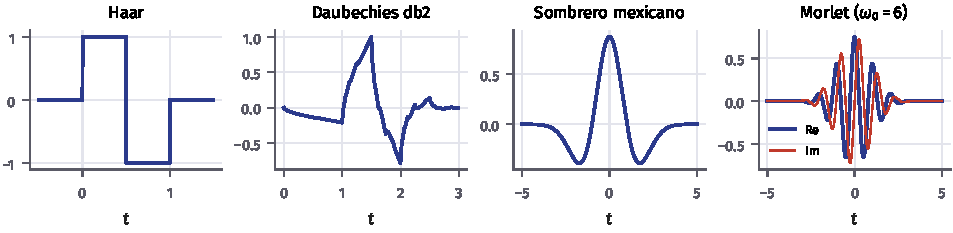
\includegraphics[width=\linewidth]{wavelets}\end{center}
  \small
  \begin{itemize}
    \item Una \alert{wavelet madre} $\psi(t)$ es una onda de duración limitada (o que decae rápido) y media nula.
    \item Se \alert{escala} con $a>0$ y se \alert{desplaza} con $b$:
    \(
      \psi_{a,b}(t)=\frac1{\sqrt a}\,\psi\!\left(\frac{t-b}a\right).
    \)
    El factor $1/\sqrt a$ mantiene la energía.
  \end{itemize}
\end{frame}

\begin{frame}{Escala y desplazamiento}
  \begin{center}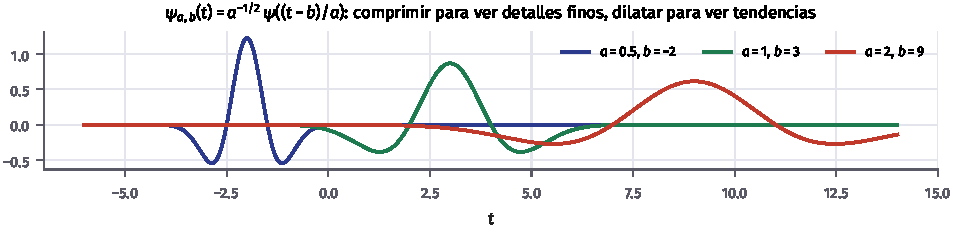
\includegraphics[width=\linewidth]{escalado_wavelet}\end{center}
  \small
  \begin{itemize}
    \item $a$ pequeño: wavelet comprimida, oscila deprisa, ve detalles finos (alta frecuencia) con buena localización en el tiempo.
    \item $a$ grande: wavelet dilatada, ve variaciones lentas (baja frecuencia) con buena resolución en frecuencia.
    \item La escala es inversa a la frecuencia: si $\psi$ oscila a $\omega_0$, $\psi_{a,b}$ oscila a $\omega_0/a$.
  \end{itemize}
\end{frame}

% =====================================================================
\section{Transformada wavelet continua}

\begin{frame}{Definición}
  \begin{definicion}[Transformada wavelet continua (CWT)]
    \[
      W_x(a,b)=\int_{-\infty}^{\infty}x(t)\,\psi_{a,b}^*(t)\dd t=\frac1{\sqrt a}\int_{-\infty}^{\infty}x(t)\,\psi^*\!\left(\frac{t-b}a\right)\dd t
    \]
  \end{definicion}
  \small
  \begin{itemize}
    \item Es la \alert{correlación} de $x$ con la wavelet escalada: mide cuánto se parece $x$ a $\psi_{a,b}$ cerca de $t=b$.
    \item Compárese con la STFT, que correla con $w(t-\tau)\e^{j\omega t}$: tres parámetros ($\tau$, $\omega$ y la longitud de ventana) frente a dos ($a$, $b$).
    \item El \alert{escalograma} es $\abs{W_x(a,b)}^2$ en el plano $(b,a)$; se suele dibujar con la frecuencia equivalente en un eje logarítmico.
    \item Para la Morlet $\psi(t)=\pi^{-1/4}\e^{j\omega_0t}\e^{-t^2/2}$, la escala $a$ (en segundos) corresponde a $f\approx\omega_0/(2\pi a)$.
  \end{itemize}
\end{frame}

\begin{frame}{Escalograma frente a espectrograma}
  \begin{center}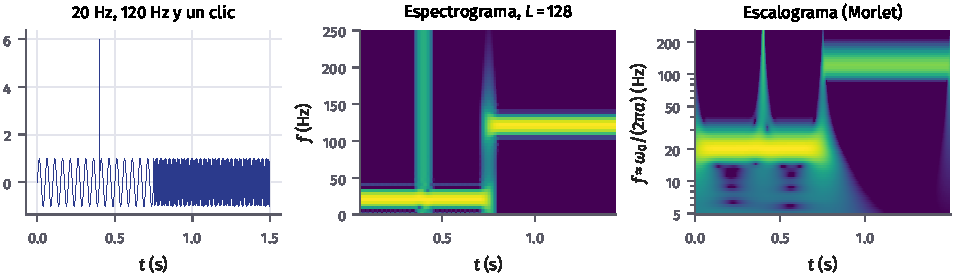
\includegraphics[width=\linewidth]{escalograma}\end{center}
  \small
  \begin{itemize}
    \item El espectrograma usa la misma ventana en todas las frecuencias: el clic se ve con la anchura de la ventana.
    \item En el escalograma el clic se estrecha al subir la frecuencia, y el tono de 20\,Hz se ve con una resolución en frecuencia más fina que el de 120\,Hz.
  \end{itemize}
  \herramienta{T5-escalograma}
\end{frame}

\begin{frame}{Condiciones sobre la wavelet}
  \small
  \begin{itemize}
    \item \alert{Admisibilidad}: con $\Psi(j\omega)$ la CTFT de $\psi$,
    \[
      C_\psi=\int_{-\infty}^{\infty}\frac{\abs{\Psi(j\omega)}^2}{\abs\omega}\dd\omega<\infty .
    \]
    Obliga a $\Psi(j0)=0$, es decir, \alert{media nula}: $\int\psi(t)\dd t=0$. Garantiza que la CWT se puede invertir:
    \[
      x(t)=\frac1{C_\psi}\int_0^\infty\!\!\int_{-\infty}^{\infty}W_x(a,b)\,\psi_{a,b}(t)\,\frac{\dd b\,\dd a}{a^2}.
    \]
    \item \alert{Momentos nulos}: $\psi$ tiene $P$ momentos nulos si $\int t^p\psi(t)\dd t=0$ para $p=0,1,\dots,P-1$. Entonces la transformada de un polinomio de grado menor que $P$ es cero: las zonas suaves dan coeficientes casi nulos y solo destacan los cambios bruscos.
    \item Haar tiene 1 momento nulo; Daubechies db$P$ tiene $P$ (con $2P$ coeficientes); el sombrero mexicano, 2.
  \end{itemize}
  \nota{En versiones anteriores la admisibilidad aparecía con $\omega$ en lugar de $\abs\omega$ en el denominador, y los momentos nulos con $p=0,\dots,N$ para «$N$ momentos».}
\end{frame}

% =====================================================================
\section{Transformada wavelet discreta}

\begin{frame}{Escalas y desplazamientos diádicos}
  \small
  \begin{itemize}
    \item La CWT es muy redundante. Basta tomar $a=2^j$ y $b=k\,2^j$, con $j,k\in\Z$:
    \[
      \psi_{j,k}(t)=2^{-j/2}\,\psi\!\left(2^{-j}t-k\right).
    \]
    \item Para algunas $\psi$ estas funciones son una \alert{base ortonormal}:
    \[
      \int_{-\infty}^{\infty}\psi_{j,k}(t)\,\psi_{j',k'}(t)\dd t=\delta[j-j']\,\delta[k-k'] .
    \]
    \item Entonces $x(t)=\sum_j\sum_k d_j[k]\,\psi_{j,k}(t)$, con coeficientes $d_j[k]=\int x(t)\psi_{j,k}(t)\dd t$, y la energía se reparte entre ellos (Parseval): $\int\abs{x}^2\dd t=\sum_{j,k}\abs{d_j[k]}^2$.
  \end{itemize}
  \nota{Las antiguas transparencias omitían el factor $2^{-j/2}$, sin el cual la base no es ortonormal, y el $\dd t$ de la integral.}
\end{frame}

\begin{frame}{Análisis multirresolución}
  \begin{columns}[c]
    \begin{column}{0.48\textwidth}
      \small
      \begin{itemize}
        \item Se añade una \alert{función de escala} $\varphi$ (la «wavelet padre»), de media 1, que recoge lo que queda por encima de la escala $2^J$.
        \item \alert{Detalle} del nivel $j$: $D_j(t)=\sum_kd_j[k]\psi_{j,k}(t)$.
        \item \alert{Aproximación} del nivel $J$: $A_J(t)=\sum_ka_J[k]\varphi_{J,k}(t)$.
        \item La señal es la aproximación más los detalles:
        \[
          x=A_J+D_J+\dots+D_1,\qquad A_{j-1}=A_j+D_j .
        \]
      \end{itemize}
    \end{column}
    \begin{column}{0.5\textwidth}
      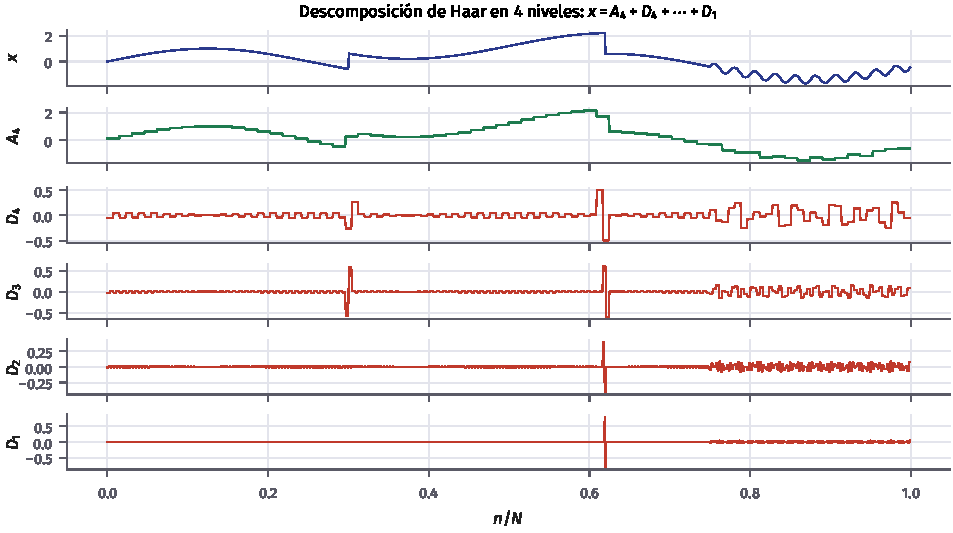
\includegraphics[width=\linewidth]{multiresolucion}
    \end{column}
  \end{columns}
  \herramienta{T5-dwt-multirresolucion}
\end{frame}

\begin{frame}{La wavelet de Haar}
  \small
  \[
    \varphi(t)=\begin{cases}1,&0\le t<1\\0,&\text{resto}\end{cases}\qquad
    \psi(t)=\begin{cases}1,&0\le t<\tfrac12\\-1,&\tfrac12\le t<1\\0,&\text{resto}\end{cases}
  \]
  \begin{columns}[T]
    \begin{column}{0.6\textwidth}
      Con una secuencia de longitud par, un nivel es:
      \[
        a_1[k]=\frac{x[2k]+x[2k+1]}{\sqrt2},\quad d_1[k]=\frac{x[2k]-x[2k+1]}{\sqrt2}.
      \]
      La inversa:
      \[
        x[2k]=\frac{a_1[k]+d_1[k]}{\sqrt2},\quad x[2k+1]=\frac{a_1[k]-d_1[k]}{\sqrt2}.
      \]
      Se repite sobre $a_1$ para obtener $a_2$ y $d_2$, y así hasta el nivel $J$.
    \end{column}
    \begin{column}{0.38\textwidth}
      \begin{ejemplo}[Un nivel a mano]
        \footnotesize
        $x=(4,6,10,12)$:
        \[
          a_1=\tfrac1{\sqrt2}(10,22),\quad d_1=\tfrac1{\sqrt2}(-2,-2).
        \]
        Energía: $16+36+100+144=296$ y $\frac{100+484+4+4}{2}=296$.
      \end{ejemplo}
    \end{column}
  \end{columns}
\end{frame}

\begin{frame}{La DWT como banco de filtros}
  \begin{columns}[c]
    \begin{column}{0.5\textwidth}
      \footnotesize
      \begin{itemize}
        \item Algoritmo de Mallat: filtrar con un paso bajo $h_0$ y un paso alto $h_1$ y \alert{diezmar por 2}:
        \begin{align*}
          a_j[k]&=\textstyle\sum_nh_0[n-2k]\,a_{j-1}[n],\\
          d_j[k]&=\textstyle\sum_nh_1[n-2k]\,a_{j-1}[n].
        \end{align*}
        \item Haar: $h_0=\frac1{\sqrt2}(1,1)$, $h_1=\frac1{\sqrt2}(1,-1)$. En general $h_1[n]=(-1)^nh_0[L-1-n]$.
        \item Cada nivel parte la banda en dos: $d_1$ ocupa $[\pi/2,\pi]$, $d_2$ $[\pi/4,\pi/2]$, …, $a_J$ $[0,\pi/2^J]$.
        \item Coeficientes: $\tfrac N2+\frac N4+\dots+\frac N{2^J}+\frac N{2^J}=N$. Coste $O(N)$.
      \end{itemize}
    \end{column}
    \begin{column}{0.48\textwidth}
      \begin{center}
        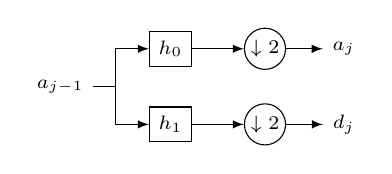
\begin{tikzpicture}[>=latex, font=\scriptsize, x=1cm, y=0.8cm]
          \node (x) at (0,0) {$a_{j-1}$};
          \node[draw] (h0) at (1.4,0.6) {$h_0$};
          \node[draw] (h1) at (1.4,-0.6) {$h_1$};
          \node[draw, circle, inner sep=1pt] (d0) at (2.6,0.6) {$\downarrow2$};
          \node[draw, circle, inner sep=1pt] (d1) at (2.6,-0.6) {$\downarrow2$};
          \node (a) at (3.6,0.6) {$a_j$};
          \node (d) at (3.6,-0.6) {$d_j$};
          \draw[->] (x) -- (0.7,0) |- (h0);
          \draw[->] (0.7,0) |- (h1);
          \draw[->] (h0) -- (d0);
          \draw[->] (h1) -- (d1);
          \draw[->] (d0) -- (a);
          \draw[->] (d1) -- (d);
        \end{tikzpicture}
      \end{center}
      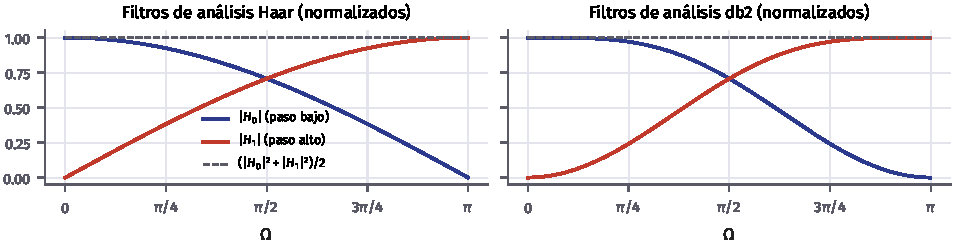
\includegraphics[width=\linewidth]{banco_filtros}
      \nota{Con $h_0$ y $h_1$ invertidos en el tiempo. $\abs{H_0}^2+\abs{H_1}^2=2$: no se pierde energía.}
    \end{column}
  \end{columns}
  \herramienta{T5-dwt-multirresolucion}
\end{frame}

\begin{frame}[t]{En código: DWT de Haar}
  \codigo[basicstyle=\ttfamily\fontsize{6.1}{6.8}\selectfont]{haar_dwt}
\end{frame}

% =====================================================================
\section{Aplicaciones}

\begin{frame}{Eliminación de ruido}
  \begin{center}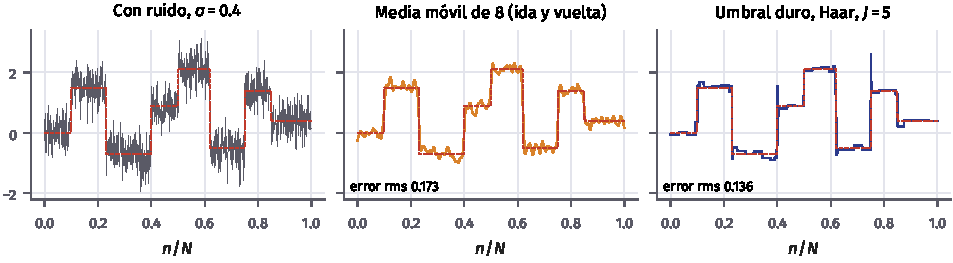
\includegraphics[width=0.88\linewidth]{eliminacion_ruido}\end{center}
  \small
  \begin{itemize}
    \item El ruido blanco reparte su energía entre todos los coeficientes; la señal la concentra en unos pocos grandes.
    \item Se \alert{anulan los coeficientes de detalle pequeños} (umbral duro) o se encogen todos (umbral suave) y se reconstruye.
    \item Umbral universal $u=\hat\sigma\sqrt{2\ln N}$, con $\hat\sigma=\operatorname{mediana}\abs{d_1}/0{,}6745$. Un paso bajo borra el ruido y también los saltos; las wavelets conservan los saltos.
  \end{itemize}
  \herramienta{T5-ruido-wavelet}
\end{frame}

\begin{frame}{En código: eliminar ruido}
  \codigo[basicstyle=\ttfamily\fontsize{6.5}{7.4}\selectfont]{eliminar_ruido}
\end{frame}

\begin{frame}{Compresión y otras aplicaciones}
  \begin{center}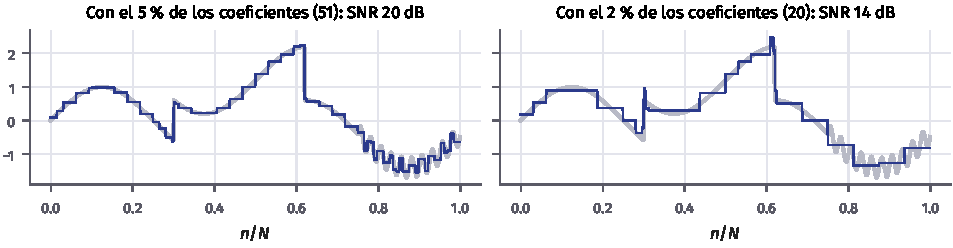
\includegraphics[width=0.85\linewidth]{compresion}\end{center}
  \small
  \begin{itemize}
    \item \alert{Compresión}: se guardan solo los coeficientes mayores. JPEG 2000 usa una DWT 2D (wavelets biortogonales 9/7) en lugar de la DCT por bloques de JPEG.
    \item \alert{Detección}: los saltos y picos dan coeficientes grandes en todas las escalas (electrocardiogramas, fallos en máquinas).
    \item \alert{Elección de la wavelet}: según la forma de lo que se busca y los momentos nulos necesarios.
  \end{itemize}
  \herramienta{T5-ruido-wavelet}
\end{frame}

% =====================================================================
\section*{Resumen}
\begin{frame}{Conceptos importantes}
  \begin{columns}[T]
    \begin{column}{0.5\textwidth}
      \begin{itemize}
        \item $\psi_{a,b}(t)=a^{-1/2}\psi((t-b)/a)$: escala inversa a la frecuencia.
        \item CWT: correlación con la wavelet escalada; escalograma.
        \item Admisible: media nula. $P$ momentos nulos anulan polinomios de grado $<P$.
      \end{itemize}
    \end{column}
    \begin{column}{0.5\textwidth}
      \begin{itemize}
        \item DWT: escalas diádicas, base ortonormal, $x=A_J+\sum D_j$.
        \item Banco de filtros $h_0$, $h_1$ con diezmado por 2; $N$ coeficientes, coste $O(N)$.
        \item Umbralizar los detalles elimina ruido y comprime.
      \end{itemize}
    \end{column}
  \end{columns}
  \bigskip
  \gris{Apuntes del Tema 5, sección 2 · Hoja de ejercicios, ejercicios 6–10.}
\end{frame}

\end{document}
